\documentclass{article}

\usepackage{graphicx}
\usepackage{tikz}
\usepackage{tikzsymbols}
\usetikzlibrary{calc,patterns,shapes.geometric}
\pagestyle{empty}
\usepackage[margin=0pt]{geometry}
\geometry{papersize={14in,12in}}

\def\centerarc[#1](#2)(#3:#4:#5){\draw[#1] ($(#2)+({#5*cos(#3)},{#5*sin(#3)})$) arc (#3:#4:#5);}

\begin{document}
	\begin{figure}
		\centering
		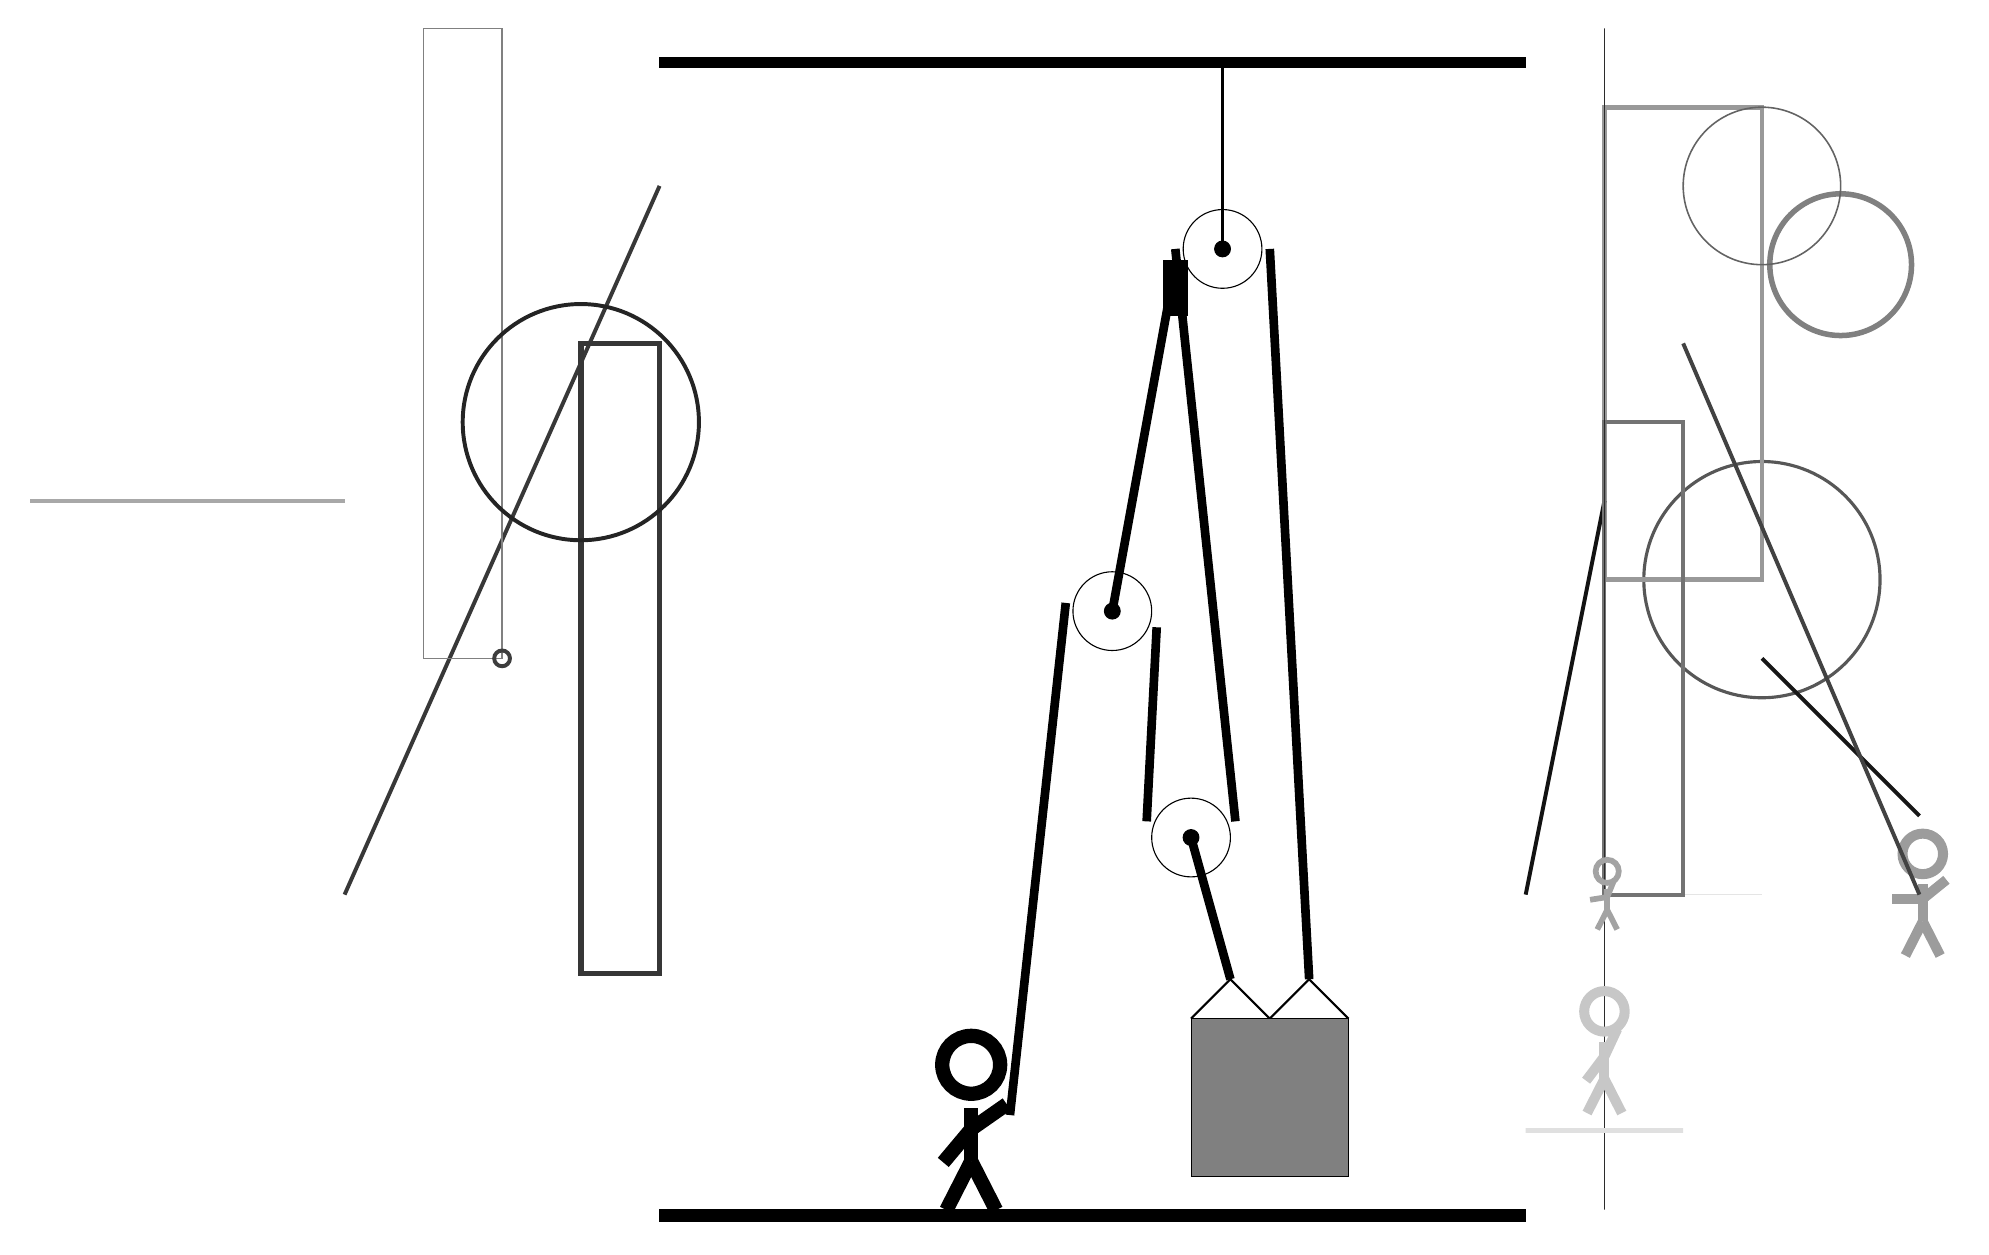
\begin{tikzpicture}
			%%%%% START %%%%%
			
			\draw[fill=black] (-6, 11.5) rectangle (5, 11.625);
			
			\draw (-0.25, 4.6) circle (0.5);
			\draw[fill=black] (-0.25, 4.6) circle (0.1);
			
			\draw (0.75, 1.725) circle (0.5);
			\draw[fill=black] (0.75, 1.725) circle (0.1);
			
			\draw (1.15, 9.2) circle (0.5);
			\draw[fill=black] (1.15, 9.2) circle (0.1);
			\draw[very thick] (1.15, 9.2) -- (1.15, 11.5);
			
			\node[line width=0.2mm, color=black!39] at (10, 1) {\Strichmaxerl[7][0][39]};
			
			\draw[line width=0.5mm, color=black!78](-6, 10) -- (-10, 1);
			\draw[line width=0.2mm, color=black!50] (-8, 12) rectangle (-9, 4);
			\draw[line width=0.7mm, color=black!79] (-6, 0) rectangle (-7, 8);
			
			\draw[line width=0.5mm, color=black!34](-10, 6) -- (-14, 6);
			\draw [line width=0.7mm, color=black!50](9, 9) circle (0.9);
			\draw [line width=0.5mm, color=black!76](-8, 4) circle (0.1);
			
			\draw [line width=0.4mm, color=black!66](8, 5) circle (1.5);
			\draw[line width=0.2mm, color=black!10] (6, 1) rectangle (8, 1);
			\draw[line width=0.6mm, color=black!40] (6, 5) rectangle (8, 11);
			
			\draw [line width=0.2mm, color=black!61](8, 10) circle (1.0);
			\draw[line width=0.5mm, color=black!91](8, 4) -- (10, 2);
			\draw[line width=0.5mm, color=black!93](5, 1) -- (6, 6);
			
			\draw[line width=0.5mm, color=black!55] (6, 1) rectangle (7, 7);
			\draw[line width=0.2mm, color=black!83] (6, 12) rectangle (6, -3);
			\draw [line width=0.5mm, color=black!86](-7, 7) circle (1.5);
			
			\node[line width=0.5mm, color=black!22] at (6, -1) {\Strichmaxerl[7][53][65]};
			
			\node[line width=0.6mm, color=black!36] at (6, 1) {\Strichmaxerl[4][9][68]};
			\draw[line width=0.5mm, color=black!74](10, 1) -- (7, 8);
			\draw[line width=0.6mm, color=black!12] (7, -2) rectangle (5, -2);
			
			\draw[thick]  (0.75, -0.575) -- (1.25, -0.075) -- (1.75, -0.575) -- (2.25, -0.075) -- (2.75, -0.575);
			\draw[fill=black!50] (0.75, -0.575) rectangle (2.75, -2.575);
			
			\draw[line width=1.1mm] (-0.25, 4.6) -- (0.55, 9.0);
			\draw[line width=1.1mm, fill=black](0.45, 8.4) rectangle (0.65, 9.0);
			\draw[line width=1.1mm] (-1.55, -1.8) -- (-0.8409, 4.7042);
			\centerarc[line width=1.1mm](-0.25, 4.6)(-20:170:0.6);
			\draw[line width=1.1mm] (0.3138, 4.3948) -- (0.1862, 1.9302);
			\centerarc[line width=1.1mm](0.75, 1.725)(160:380:0.6);
			\draw[line width=1.1mm] (1.3138, 1.9302) -- (0.55, 9.2);
			\draw[line width=1.1mm](0.75, 1.725) -- (1.25, -0.075);
			\centerarc[line width=1.1mm](1.15, 9.2)(0:180:0.6);
			\draw[line width=1.1mm] (1.75, 9.2) -- (2.25, -0.075);
			
			\node at (-2, -1.9) {\Strichmaxerl[10][50][35]};
			
			\draw[fill=black] (-6, -3) rectangle (5, -3.15);
			
			%%%%% END %%%%%
		\end{tikzpicture}
	\end{figure}	
\end{document}